% % !TeX root = ../main_en.tex

% \chapter{Contexte}

% Ce chapitre introduit les notions nécessaires pour comprendre la suite du rapport. 
% L'objectif est de fixer le contexte général : ce qu'est un réseau convolutionnel, pourquoi la robustesse est une 
% question importante, et en quoi les perturbations adversariales motivent l'analyse menée dans ce travail.

% \section{Les réseaux convolutionnels en vision par ordinateur}

% En vision par ordinateur, une image peut être vue comme une grille de pixels. 
% Chaque pixel contient une information visuelle locale saisie par un capteur tel qu'un appareil photo, comme une intensité 
% lumineuse, dans le cas d'une image en niveaux de gris (image en noir et blanc) ou plusieurs valeurs dans le cas d'une image couleur, par exemple les canaux rouge, vert et bleu.
% Un modèle de classification d'images doit donc apprendre à transformer cette grille de valeurs en une prédiction, 
% comme une classe d'objet (par exemple, "chat" ou "chien") ou une catégorie visuelle (par exemple, "animal" ou "véhicule").

% Les réseaux de neurones convolutionnels, contrairement à un réseau entièrement 
% connecté (\textit{fully-connected}), qui traiterait tous les pixels comme des variables 
% indépendantes, exploite directement la structure spatiale de l'image. 
% Il analyse l'image localement, à l'aide de filtres appliqués sur de petites régions voisines, afin de détecter des motifs locaux comme des contours ou des textures. 
% En combinant ces motifs à travers plusieurs couches, le CNN peut construire des représentations de plus en plus abstraites,
% capables de reconnaître des objets complexes ou des catégories visuelles. La figure~\ref{fig:lenet5} illustre justement ce principe.

% \begin{figure}[H]
%     \centering
%     \resizebox{\textwidth}{!}{
%         \begin{tikzpicture}[
%             font=\sffamily\small,
%             map/.style={fill=gray!60, draw=gray!80, line width=0.5pt},
%             vector/.style={fill=gray!70, draw=none},
%             conn/.style={draw=black, thin},
%             rf/.style={draw=black, thick, fill=none}
%         ]
%     \filldraw[fill=gray!40, draw=none] (0,0) rectangle (3.2, 3.2);
%     \draw[line width=4pt, rotate around={15:(1.6,1.7)}] (1.6, 1.7) ellipse (0.7 and 1.1);
%     \node[above, align=center, font=\sffamily\small\bfseries] at (1.6, 3.8) {INPUT\\32x32};
%     \foreach \i in {5,4,...,0} {

%         \filldraw[map] (5.0 - \i*0.15, 0.2 + \i*0.15) rectangle +(2.8, 2.8);

%     }

%     \node[above, align=center] at (6.0, 3.8) {C1: feature maps\\6@28x28};
%     \foreach \i in {5,4,...,0} {

%         \filldraw[map] (9.0 - \i*0.15, 0.6 + \i*0.15) rectangle +(1.4, 1.4);

%     }
%     \node[above, align=center] at (9.3, 3.8) {S2: f. maps\\6@14x14};
%     \foreach \i in {15,14,...,0} {

%         \filldraw[map] (12.5 - \i*0.1, 0.8 + \i*0.1) rectangle +(1.0, 1.0);

%     }
%     \node[above, align=center] at (12.2, 3.8) {C3: f. maps\\16@10x10};
%     \foreach \i in {15,14,...,0} {

%         \filldraw[map] (15.5 - \i*0.1, 1.0 + \i*0.1) rectangle +(0.5, 0.5);

%     }
%     \node[above, align=center] at (15.0, 3.8) {S4: f. maps\\16@5x5};
%     \filldraw[vector] (18.5, 0.5) -- (18.9, 0.5) -- (16.9, 3.5) -- (16.5, 3.5) -- cycle;
%     \node[above, align=center] at (17.7, 3.8) {C5: layer\\120};
%     \filldraw[vector] (21.5, 0.7) -- (21.9, 0.7) -- (20.3, 3.1) -- (19.9, 3.1) -- cycle;
%     \node[above, align=center] at (20.9, 3.8) {F6: layer\\84};
%     \filldraw[vector] (24.5, 1.0) -- (24.9, 1.0) -- (23.9, 2.4) -- (23.5, 2.4) -- cycle;
%     \node[above, align=center] at (24.2, 3.8) {OUTPUT\\10};
%     \draw[rf] (2.1, 0.4) rectangle (2.9, 1.2);
%     \draw[rf] (7.2, 0.4) rectangle (7.4, 0.6);
%     \draw[conn] (2.1, 0.4) -- (7.2, 0.4);
%     \draw[conn] (2.9, 0.4) -- (7.4, 0.4);
%     \draw[conn] (2.1, 1.2) -- (7.2, 0.6);
%     \draw[conn] (2.9, 1.2) -- (7.4, 0.6);
%     \draw[rf] (5.8, 1.2) rectangle (6.2, 1.6);
%     \draw[rf] (9.4, 1.1) rectangle (9.6, 1.3);
%     \draw[conn] (5.8, 1.2) -- (9.4, 1.1);
%     \draw[conn] (6.2, 1.2) -- (9.6, 1.1);
%     \draw[conn] (5.8, 1.6) -- (9.4, 1.3);
%     \draw[conn] (6.2, 1.6) -- (9.6, 1.3);
%     \draw[rf] (9.9, 0.7) rectangle (10.2, 1.0);
%     \draw[rf] (13.1, 0.85) rectangle (13.3, 1.05);
%     \draw[conn] (9.9, 0.7) -- (13.1, 0.85);
%     \draw[conn] (10.2, 0.7) -- (13.3, 0.85);
%     \draw[conn] (9.9, 1.0) -- (13.1, 1.05);
%     \draw[conn] (10.2, 1.0) -- (13.3, 1.05);
%     \draw[rf] (12.7, 1.3) rectangle (12.9, 1.5);
%     \draw[rf] (15.6, 1.25) rectangle (15.7, 1.35);
%     \draw[conn] (12.7, 1.3) -- (15.6, 1.25);
%     \draw[conn] (12.9, 1.3) -- (15.7, 1.25);
%     \draw[conn] (12.7, 1.5) -- (15.6, 1.35);
%     \draw[conn] (12.9, 1.5) -- (15.7, 1.35);
%     \draw[rf] (17.7, 1.7) rectangle (17.9, 1.9);
%     \draw[conn] (15.5, 1.0) -- (17.7, 1.7); % De l'avant-bas de S4
%     \draw[conn] (14.0, 3.0) -- (17.7, 1.9); % De l'arrière-haut de S4
%     \draw[conn] (16.9, 3.5) -- (20.3, 3.1);
%     \draw[conn] (17.9, 2.0) -- (21.1, 1.9);
%     \draw[conn] (18.9, 0.5) -- (21.9, 0.7);
%     \draw[conn] (20.3, 3.1) -- (23.9, 2.4);
%     \draw[conn] (21.1, 1.9) -- (24.4, 1.7);
%     \draw[conn] (21.9, 0.7) -- (24.9, 1.0);
%     \def\tickH{-0.2}
%     \def\tickL{-0.6}
%     \def\textY{-0.9}
%     \draw[conn] (6.0, \tickH) -- (6.0, \tickL);
%     \node[below, align=center] at (6.0, \textY) {Convolutions};
%     \draw[conn] (9.3, \tickH) -- (9.3, \tickL);
%     \node[below, align=center] at (9.3, \textY) {Subsampling};
%     \draw[conn] (12.2, \tickH) -- (12.2, \tickL);
%     \node[below, align=center] at (12.2, \textY) {Convolutions};
%     \draw[conn] (15.0, \tickH) -- (15.0, \tickL);
%     \node[below, align=center] at (15.0, \textY) {Subsampling};
%     \draw[conn] (17.7, \tickH) -- (17.7, \tickL);
%     \node[below, align=center] at (17.7, \textY) {Full connection};
%     \draw[conn] (20.9, \tickH) -- (20.9, \tickL);
%     \node[below, align=center] at (20.9, \textY) {Full connection};
%     \draw[conn] (24.2, \tickH) -- (24.2, \tickL);
%     \node[below, align=center] at (24.2, \textY) {Gaussian connections};
%         \end{tikzpicture}
%     }
%     \caption{Architecture du réseau de neurones convolutionnel LeNet-5. Adapté de \cite{lecun1998gradient}.}
%     \label{fig:lenet5}
% \end{figure}

% L'output de taille $10$ correspond à une prédiction de classe parmi $10$ classes possibles, 
% ici cela représente les chiffres de 0 à 9.

% \section{Robustesse des modèles de vision}

% La performance d'un modèle est souvent mesurée sur des images propres, issues du même dataset que les données d'entraînement.
% Dans ce cadre, on évalue généralement si le modèle donne la bonne classe pour chaque image, ainsi plus le modèle prédit la bonne
% classe plus il est performant.

% En pratique, une image peut subir de nombreuses variations : un léger bruit, un changement de contraste, etc.
% Pour un observateur humain, ces changements ne modifient pas nécessairement le contenu de l'image. 
% Un chat reste un chat même si l'image est un peu bruitée ou légèrement plus sombre. 
% On attend donc d'un modèle robuste qu'il conserve une prédiction cohérente face à des variations.

% La robustesse désigne cette capacité à maintenir un comportement stable lorsque l'entrée est modifiée.   

% \section{Perturbations adversariales}
% \label{sec:perturbation_adversariale}

% Une perturbation adversariale est une modification volontairement choisie pour tromper un modèle, tout en restant imperceptible pour l'oeil humain~\cite{szegedy2014intriguing}. 
% L'idée n'est pas simplement d'ajouter un bruit (variation aléatoire de la valeur de ses pixels) quelconque à l'image,
% mais de construire une perturbation qui provoque un changement de prédiction. 

% On peut représenter ce principe de manière simple. 
% À partir d'une image $x$, on construit une image modifiée
% \[
%     \widetilde{x} = x + \delta,
% \]
% où $\delta$ désigne la perturbation ajoutée. 

% Ces perturbations peuvent être étudiées sous plusieurs angles. 
% Dans ce rapport, nous nous intéressons aux perturbations qui nous permettent de mieux comprendre quelles 
% directions de l'espace des images influencent fortement le comportement du modèle.

% \section{Perturbations universelles et directions de vulnérabilité}

% Dans le cas le plus simple, une perturbation adversariale est construite pour une image donnée. 
% Par conséquent une dépendance forte entre l'image et la perturbation se crée, ainsi la perturbation a moins de
% chance de tromper le modèle sur une autre image.
% En revanche, si la perturbation est construite à partir d'une vulnérabilité propre au réseau, elle ne dépend plus uniquement d'une image spécifique. 
% Elle devient alors liée à certaines directions sensibles du modèle, des directions qui sont elles-mêmes façonnées par les données, 
% la dynamique d'entraînement, les non-linéarités et la géométrie de la frontière de décision.
% Une même perturbation peut donc être réutilisée sur plusieurs images différentes et, dans certains cas, tromper le modèle de manière répétée.

% C'est précisément ce que l'on appelle une perturbation adversariale universelle~\cite{moosavi2017universal}.

% Si l'on considère une image comme un point dans un espace de grande dimension, alors une perturbation correspond à un déplacement dans cet espace. 
% Certaines directions peuvent être presque sans effet sur la prédiction, tandis que d'autres peuvent modifier fortement la sortie du réseau comme illustré par la figure~\ref{fig:vulnerabilite_realiste}.

% \begin{figure}[H]
%     \centering
%     \begin{tikzpicture}[scale=1.1, font=\sffamily]

%         \definecolor{class0}{HTML}{EBF5FB} 
%         \definecolor{class9}{HTML}{FDEDEC} 
%         \definecolor{accentblue}{HTML}{21618C}
%         \definecolor{accentred}{HTML}{CB4335}
%         \definecolor{accentgreen}{HTML}{27AE60}

%         \fill[class0]  (3,3) -- (4,2) -- (6,2) -- (7.5,3.5) -- (8,5) -- (6.5,6.5) -- (5,6.5) -- (3.5,6) -- (2,4.5) -- cycle;
%         \fill[gray!15] (10,2) -- (10,6) -- (8,5) -- (7.5,3.5) -- cycle; 
%         \fill[gray!5]  (8,8) -- (5,8) -- (5,6.5) -- (6.5,6.5) -- cycle; 
%         \fill[gray!15] (5,8) -- (2,8) -- (3.5,6) -- (5,6.5) -- cycle; 
%         \fill[gray!5]  (2,8) -- (0,8) -- (0,6) -- (2,4.5) -- (3.5,6) -- cycle; 
%         \fill[gray!15] (0,6) -- (0,2) -- (3,3) -- (2,4.5) -- cycle; 
%         \fill[gray!5]  (0,2) -- (0,0) -- (3,0) -- (4,2) -- (3,3) -- cycle; 
%         \fill[gray!15] (3,0) -- (7,0) -- (6,2) -- (4,2) -- cycle; 
%         \fill[gray!5]  (7,0) -- (10,0) -- (10,2) -- (7.5,3.5) -- (6,2) -- cycle; 
%         \fill[class9]  (10,6) -- (10,8) -- (8,8) -- (6.5,6.5) -- (8,5) -- cycle; 

%         \draw[gray, thick] (3,3) -- (4,2) -- (6,2) -- (7.5,3.5) -- (8,5) -- (6.5,6.5) -- (5,6.5) -- (3.5,6) -- (2,4.5) -- cycle;
%         \draw[gray, thick] (3,3) -- (0,2);
%         \draw[gray, thick] (4,2) -- (3,0);
%         \draw[gray, thick] (6,2) -- (7,0);
%         \draw[gray, thick] (7.5,3.5) -- (10,2);
%         \draw[gray, thick] (8,5) -- (10,6);
%         \draw[gray, thick] (6.5,6.5) -- (8,8);
%         \draw[gray, thick] (5,6.5) -- (5,8);
%         \draw[gray, thick] (3.5,6) -- (2,8);
%         \draw[gray, thick] (2,4.5) -- (0,6);
%         \draw[gray, thick] (0,0) rectangle (10,8);

%         \node[accentblue, font=\bfseries\huge] at (4.2, 4.2) {0};
%         \node[accentred, font=\bfseries\huge] at (8.5, 7.3) {9};
%         \foreach \p/\l in {(9,4)/1, (6.5,7.3)/2, (3.5,7.3)/3, (1.2,6.8)/4, (1.2,4)/5, (1.8,1)/6, (5,0.8)/7, (8.5,1.2)/8}
%             \node[gray, font=\bfseries\Large] at \p {\l};

%         \coordinate (X) at (6.8, 5.8);
%         \filldraw[black] (X) circle (2.5pt) node[left, xshift=-2pt] {$x$};
        
%         \coordinate (X_safe) at (5.8, 5.1);
%         \draw[accentgreen, ->, >=stealth, very thick] (X) -- (X_safe) node[midway, sloped, below] {$\eta_1$};
%         \filldraw[accentgreen] (X_safe) circle (2pt) node[below left, font=\footnotesize] {Toujours classé 0};

%         \coordinate (X_adv) at (7.4, 6.4);
%         \draw[accentred, ->, >=stealth, very thick] (X) -- (X_adv) node[midway, sloped, above] {$\eta_{adv}$};
%         \filldraw[accentred] (X_adv) circle (2pt) node[below right, font=\footnotesize] {Classé en 9 !};

%         \begin{scope}[shift={(0,-3)}]
%             \draw[gray!30, fill=white] (-0.5, 0) rectangle (11.3, 2.2);
            
%             \filldraw[black] (0.5, 1.8) circle (2pt);
%             \node[right, font=\small] at (0.8, 1.8) {Image originale ($x$)};
            
%             \fill[class0] (0.5, 1.0) rectangle (0.9, 1.3);
%             \draw[gray, thin] (0.5, 1.0) rectangle (0.9, 1.3);
%             \node[right, font=\small] at (1.0, 1.15) {Région de confiance (Classe 0)};
            
%             \fill[class9] (0.5, 0.3) rectangle (0.9, 0.6);
%             \draw[gray, thin] (0.5, 0.3) rectangle (0.9, 0.6);
%             \node[right, font=\small] at (1.0, 0.45) {Région d'erreur (Classe 9)};
            
%             \draw[accentgreen, ->, >=stealth, thick] (5.5, 1.45) -- (6.3, 1.45);
%             \node[right, font=\small] at (6.5, 1.45) {$\eta_1$ : Perturbation inoffensive};
            
%             \draw[accentred, ->, >=stealth, thick] (5.5, 0.75) -- (6.3, 0.75);
%             \node[right, font=\small] at (6.5, 0.75) {$\eta_{adv}$ : Direction de vulnérabilité};
%         \end{scope}

%     \end{tikzpicture}
%     \caption{Illustration du concept de direction de vulnérabilité.}
%     \label{fig:vulnerabilite_realiste}
% \end{figure}



% !TeX root = ../main_en.tex

\chapter{Background}

This chapter establishes the concepts needed for the rest of the report: CNNs as convolution-based models, robustness as prediction stability,
and adversarial perturbations as directions in image space.

\section{Convolutional Networks in Computer Vision}

A digital image can be viewed as a tensor $X \in \mathbb{R}^{C \times H \times W}$, where $C$ denotes the color channels and $H,W$
the spatial dimensions. A classifier learns a function
\[
    f : \mathbb{R}^{C \times H \times W} \longrightarrow \{1,\ldots,K\},
\]
that assigns each image to one of $K$ categories.

Convolutional networks exploit the spatial structure of images. Unlike a fully connected layer, a convolution
applies the same local filter at every position. This weight sharing enables a pattern, such as an edge or a texture, to be detected regardless of its position.

By stacking several layers, the network combines local patterns into more abstract representations. The first layers capture
simple structures, while deeper layers produce information more closely related to objects. Figure~\ref{fig:lenet5} illustrates this principle.

\begin{figure}[H]
    \centering
    \resizebox{\textwidth}{!}{
        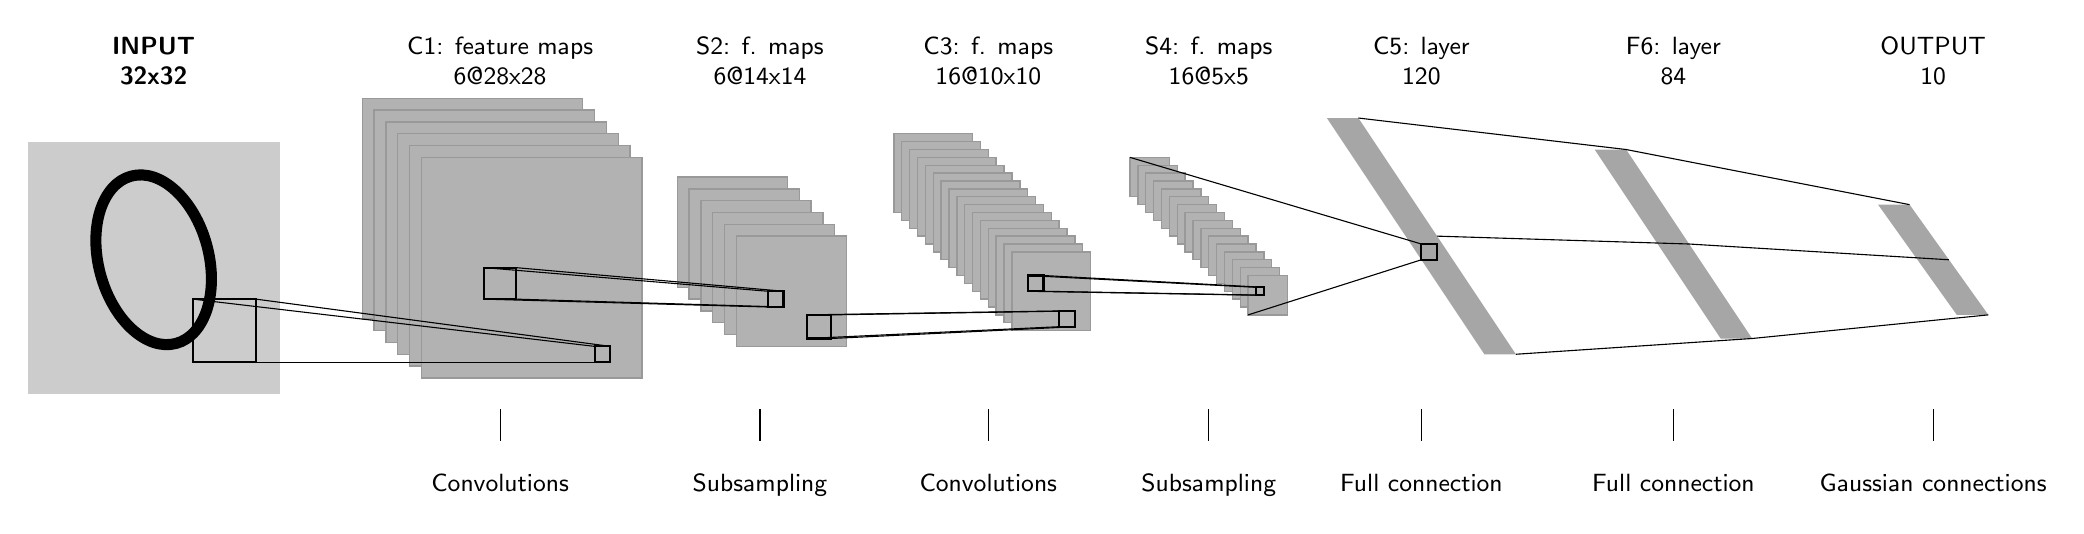
\begin{tikzpicture}[
            font=\sffamily\small,
            map/.style={fill=gray!60, draw=gray!80, line width=0.5pt},
            vector/.style={fill=gray!70, draw=none},
            conn/.style={draw=black, thin},
            rf/.style={draw=black, thick, fill=none}
        ]
    \filldraw[fill=gray!40, draw=none] (0,0) rectangle (3.2, 3.2);
    \draw[line width=4pt, rotate around={15:(1.6,1.7)}] (1.6, 1.7) ellipse (0.7 and 1.1);
    \node[above, align=center, font=\sffamily\small\bfseries] at (1.6, 3.8) {INPUT\\32x32};
    \foreach \i in {5,4,...,0} {

        \filldraw[map] (5.0 - \i*0.15, 0.2 + \i*0.15) rectangle +(2.8, 2.8);

    }

    \node[above, align=center] at (6.0, 3.8) {C1: feature maps\\6@28x28};
    \foreach \i in {5,4,...,0} {

        \filldraw[map] (9.0 - \i*0.15, 0.6 + \i*0.15) rectangle +(1.4, 1.4);

    }
    \node[above, align=center] at (9.3, 3.8) {S2: f. maps\\6@14x14};
    \foreach \i in {15,14,...,0} {

        \filldraw[map] (12.5 - \i*0.1, 0.8 + \i*0.1) rectangle +(1.0, 1.0);

    }
    \node[above, align=center] at (12.2, 3.8) {C3: f. maps\\16@10x10};
    \foreach \i in {15,14,...,0} {

        \filldraw[map] (15.5 - \i*0.1, 1.0 + \i*0.1) rectangle +(0.5, 0.5);

    }
    \node[above, align=center] at (15.0, 3.8) {S4: f. maps\\16@5x5};
    \filldraw[vector] (18.5, 0.5) -- (18.9, 0.5) -- (16.9, 3.5) -- (16.5, 3.5) -- cycle;
    \node[above, align=center] at (17.7, 3.8) {C5: layer\\120};
    \filldraw[vector] (21.5, 0.7) -- (21.9, 0.7) -- (20.3, 3.1) -- (19.9, 3.1) -- cycle;
    \node[above, align=center] at (20.9, 3.8) {F6: layer\\84};
    \filldraw[vector] (24.5, 1.0) -- (24.9, 1.0) -- (23.9, 2.4) -- (23.5, 2.4) -- cycle;
    \node[above, align=center] at (24.2, 3.8) {OUTPUT\\10};
    \draw[rf] (2.1, 0.4) rectangle (2.9, 1.2);
    \draw[rf] (7.2, 0.4) rectangle (7.4, 0.6);
    \draw[conn] (2.1, 0.4) -- (7.2, 0.4);
    \draw[conn] (2.9, 0.4) -- (7.4, 0.4);
    \draw[conn] (2.1, 1.2) -- (7.2, 0.6);
    \draw[conn] (2.9, 1.2) -- (7.4, 0.6);
    \draw[rf] (5.8, 1.2) rectangle (6.2, 1.6);
    \draw[rf] (9.4, 1.1) rectangle (9.6, 1.3);
    \draw[conn] (5.8, 1.2) -- (9.4, 1.1);
    \draw[conn] (6.2, 1.2) -- (9.6, 1.1);
    \draw[conn] (5.8, 1.6) -- (9.4, 1.3);
    \draw[conn] (6.2, 1.6) -- (9.6, 1.3);
    \draw[rf] (9.9, 0.7) rectangle (10.2, 1.0);
    \draw[rf] (13.1, 0.85) rectangle (13.3, 1.05);
    \draw[conn] (9.9, 0.7) -- (13.1, 0.85);
    \draw[conn] (10.2, 0.7) -- (13.3, 0.85);
    \draw[conn] (9.9, 1.0) -- (13.1, 1.05);
    \draw[conn] (10.2, 1.0) -- (13.3, 1.05);
    \draw[rf] (12.7, 1.3) rectangle (12.9, 1.5);
    \draw[rf] (15.6, 1.25) rectangle (15.7, 1.35);
    \draw[conn] (12.7, 1.3) -- (15.6, 1.25);
    \draw[conn] (12.9, 1.3) -- (15.7, 1.25);
    \draw[conn] (12.7, 1.5) -- (15.6, 1.35);
    \draw[conn] (12.9, 1.5) -- (15.7, 1.35);
    \draw[rf] (17.7, 1.7) rectangle (17.9, 1.9);
    \draw[conn] (15.5, 1.0) -- (17.7, 1.7); % De l'avant-bas de S4
    \draw[conn] (14.0, 3.0) -- (17.7, 1.9); % De l'arrière-haut de S4
    \draw[conn] (16.9, 3.5) -- (20.3, 3.1);
    \draw[conn] (17.9, 2.0) -- (21.1, 1.9);
    \draw[conn] (18.9, 0.5) -- (21.9, 0.7);
    \draw[conn] (20.3, 3.1) -- (23.9, 2.4);
    \draw[conn] (21.1, 1.9) -- (24.4, 1.7);
    \draw[conn] (21.9, 0.7) -- (24.9, 1.0);
    \def\tickH{-0.2}
    \def\tickL{-0.6}
    \def\textY{-0.9}
    \draw[conn] (6.0, \tickH) -- (6.0, \tickL);
    \node[below, align=center] at (6.0, \textY) {Convolutions};
    \draw[conn] (9.3, \tickH) -- (9.3, \tickL);
    \node[below, align=center] at (9.3, \textY) {Subsampling};
    \draw[conn] (12.2, \tickH) -- (12.2, \tickL);
    \node[below, align=center] at (12.2, \textY) {Convolutions};
    \draw[conn] (15.0, \tickH) -- (15.0, \tickL);
    \node[below, align=center] at (15.0, \textY) {Subsampling};
    \draw[conn] (17.7, \tickH) -- (17.7, \tickL);
    \node[below, align=center] at (17.7, \textY) {Full connection};
    \draw[conn] (20.9, \tickH) -- (20.9, \tickL);
    \node[below, align=center] at (20.9, \textY) {Full connection};
    \draw[conn] (24.2, \tickH) -- (24.2, \tickL);
    \node[below, align=center] at (24.2, \textY) {Gaussian connections};
        \end{tikzpicture}
    }
    \caption{Architecture of the LeNet-5 convolutional neural network. Adapted from \cite{lecun1998gradient}.}
    \label{fig:lenet5}
\end{figure}

The output of size $10$ here corresponds to a prediction among the ten possible digits.

\section{Robustness of Vision Models}

Performance is often measured on clean images similar to those used during training. This measure is insufficient: a model can be accurate yet unstable under small variations.

Consider an image $x$ and a perturbation $\delta$. A model is locally robust if its prediction remains stable when $x$ is replaced by $x+\delta$:
\[
    f(x+\delta) = f(x)
    \qquad \text{for perturbations } \delta \text{ that are sufficiently small.}
\]

\section{Adversarial Perturbations}
\label{sec:perturbation_adversariale}

An adversarial perturbation is a modification chosen to change a model's prediction while remaining small or barely visible to the human eye~\cite{szegedy2014intriguing}. It is not random noise: it follows a direction that strongly influences the network's output.

Starting from an image $x$, we construct a perturbed image
\[
    \widetilde{x} = x + \delta,
\]
with a perturbation $\delta$ that is sufficiently small but satisfies
\[
    f(\widetilde{x}) \neq f(x).
\]
In this report, these perturbations primarily serve as an analytical tool: they indicate which directions in image space are strongly amplified by the model.

\section{Universal Perturbations and Directions of Vulnerability}

In the simplest case, an adversarial perturbation is constructed for a given image and therefore depends strongly on that image.

A universal adversarial perturbation is based on a stronger idea: finding a single perturbation $\delta$ that can be added to many
different images~\cite{moosavi2017universal}.

Such a perturbation therefore exploits more than a particular feature of a specific image. It exploits a sensitive direction of the model, related to the learned weights,
the data, and nonlinearities, but also to the structure of the architecture. This last point motivates the present report.

If an image is viewed as a point in a high-dimensional space, a perturbation is a displacement. Some directions have little effect,
whereas others quickly cross a decision boundary, as illustrated in Figure~\ref{fig:vulnerabilite_universelle_exacte}.

\begin{figure}[H]
    \centering
    \resizebox{\linewidth}{!}{%
    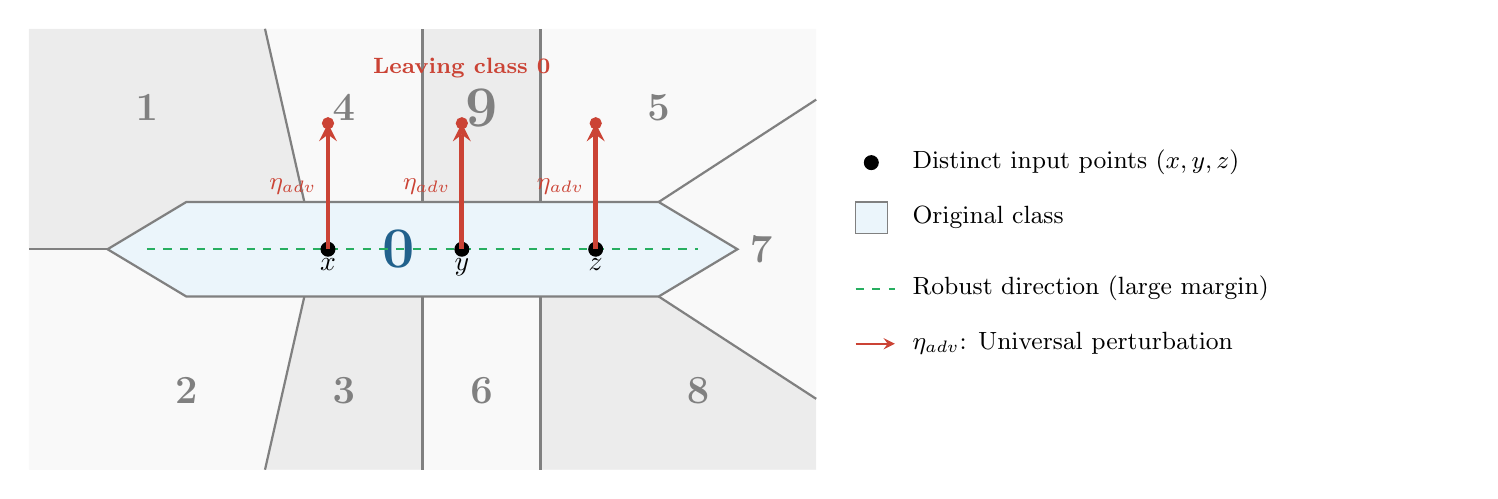
\begin{tikzpicture}[scale=1, font=\sffamily]

        \definecolor{class0}{HTML}{EBF5FB} 
        \definecolor{accentblue}{HTML}{21618C}
        \definecolor{accentred}{HTML}{CB4335}
        \definecolor{accentgreen}{HTML}{27AE60}
        \coordinate (C_L)  at (1.0, 4);
        \coordinate (C_TL) at (2.0, 4.6);
        \coordinate (C_TR) at (8.0, 4.6);
        \coordinate (C_R)  at (9.0, 4);
        \coordinate (C_BR) at (8.0, 3.4);
        \coordinate (C_BL) at (2.0, 3.4);
        \coordinate (T1) at (3.5, 4.6); \coordinate (R_T1) at (3.0, 6.8);
        \coordinate (T2) at (5.0, 4.6); \coordinate (R_T2) at (5.0, 6.8);
        \coordinate (T3) at (6.5, 4.6); \coordinate (R_T3) at (6.5, 6.8);
        \coordinate (B1) at (3.5, 3.4); \coordinate (R_B1) at (3.0, 1.2);
        \coordinate (B2) at (5.0, 3.4); \coordinate (R_B2) at (5.0, 1.2);
        \coordinate (B3) at (6.5, 3.4); \coordinate (R_B3) at (6.5, 1.2);
        \coordinate (R_R1) at (10, 5.9);
        \coordinate (R_R2) at (10, 2.1);
        \coordinate (R_L)  at (0, 4); 

        \fill[gray!5] (0,1.2) rectangle (10,6.8);
        \fill[gray!15] (C_TL) -- (C_L) -- (R_L) -- (0,6.8) -- (R_T1) -- (T1) -- cycle; 
        \fill[gray!5]  (T1) -- (R_T1) -- (R_T2) -- (T2) -- cycle;            
        \fill[gray!15] (T2) -- (R_T2) -- (R_T3) -- (T3) -- cycle;            
        \fill[gray!5]  (T3) -- (R_T3) -- (10,6.8) -- (R_R1) -- (C_TR) -- cycle;
        \fill[gray!5] (C_TR) -- (R_R1) -- (10,2.1) -- (R_R2) -- (C_BR) -- (C_R) -- cycle;
        \fill[gray!15] (C_BR) -- (R_R2) -- (10,1.2) -- (R_B3) -- (B3) -- cycle;
        \fill[gray!5]  (B3) -- (R_B3) -- (R_B2) -- (B2) -- cycle;            
        \fill[gray!15] (B2) -- (R_B2) -- (R_B1) -- (B1) -- cycle;            
        \fill[gray!5]  (B1) -- (R_B1) -- (0,1.2) -- (R_L) -- (C_L) -- (C_BL) -- cycle; 
        \fill[class0] (C_L) -- (C_TL) -- (C_TR) -- (C_R) -- (C_BR) -- (C_BL) -- cycle;

        \draw[gray, thick] (C_L) -- (C_TL) -- (C_TR) -- (C_R) -- (C_BR) -- (C_BL) -- cycle;
        \draw[gray, thick] (C_L) -- (R_L); 
        \draw[gray, thick] (T1) -- (R_T1);
        \draw[gray, thick] (T2) -- (R_T2);
        \draw[gray, thick] (T3) -- (R_T3);
        \draw[gray, thick] (C_TR) -- (R_R1);
        \draw[gray, thick] (C_BR) -- (R_R2);
        \draw[gray, thick] (B3) -- (R_B3);
        \draw[gray, thick] (B2) -- (R_B2);
        \draw[gray, thick] (B1) -- (R_B1);

        \node[accentblue, font=\bfseries\huge] at (4.7, 4) {0};
        \node[gray, font=\bfseries\huge] at (5.75, 5.8) {9};
        \node[gray, font=\bfseries\Large] at (1.5, 5.8) {1};
        \node[gray, font=\bfseries\Large] at (4.0, 5.8) {4};
        \node[gray, font=\bfseries\Large] at (8.0, 5.8) {5};
        \node[gray, font=\bfseries\Large] at (9.3, 4.0) {7};
        \node[gray, font=\bfseries\Large] at (8.5, 2.2) {8};
        \node[gray, font=\bfseries\Large] at (5.75, 2.2) {6};
        \node[gray, font=\bfseries\Large] at (4.0, 2.2) {3};
        \node[gray, font=\bfseries\Large] at (2.0, 2.2) {2};

        \draw[accentgreen, thick, dashed] (1.5, 4) -- (8.5, 4);

        \coordinate (X1) at (3.8, 4);
        \coordinate (X2) at (5.5, 4);
        \coordinate (X3) at (7.2, 4);

        \filldraw[black] (X1) circle (2.5pt) node[below] {$x$};
        \filldraw[black] (X2) circle (2.5pt) node[below] {$y$};
        \filldraw[black] (X3) circle (2.5pt) node[below] {$z$};

        \draw[accentred, ->, >=stealth, line width=1.8pt] (X1) -- +(0, 1.6) node[midway, left, font=\small] {$\eta_{adv}$};
        \draw[accentred, ->, >=stealth, line width=1.8pt] (X2) -- +(0, 1.6) node[midway, left, font=\small] {$\eta_{adv}$};
        \draw[accentred, ->, >=stealth, line width=1.8pt] (X3) -- +(0, 1.6) node[midway, left, font=\small] {$\eta_{adv}$};

        \filldraw[accentred] (3.8, 5.6) circle (2pt);
        \filldraw[accentred] (5.5, 5.6) circle (2pt);
        \filldraw[accentred] (7.2, 5.6) circle (2pt);
        
        \node[accentred, font=\footnotesize\bfseries, inner sep=2pt] at (5.5, 6.3) {Leaving class 0};

        \begin{scope}[shift={(10.5, 2.5)}]
            \fill[white] (-0.2, -0.1) rectangle (7.8, 3.1);
            
            \filldraw[black] (0.2, 2.6) circle (2.5pt);
            \node[right, font=\small] at (0.6, 2.6) {Distinct input points ($x, y, z$)};
            
            \fill[class0] (0, 1.7) rectangle (0.4, 2.1);
            \draw[gray, thin] (0, 1.7) rectangle (0.4, 2.1);
            \node[right, font=\small] at (0.6, 1.9) {Original class};

            \draw[accentgreen, thick, dashed] (0, 1.0) -- (0.5, 1.0);
            
            \node[right, font=\small] at (0.6, 1.0) {Robust direction (large margin)};
            
            \draw[accentred, ->, >=stealth, thick] (0, 0.3) -- (0.5, 0.3);
            \node[right, font=\small] at (0.6, 0.3) {$\eta_{adv}$: Universal perturbation};
        \end{scope}

    \end{tikzpicture}
    }
    \caption{Illustration of a universal perturbation in an anisotropic decision region.
    The same perturbation direction $\eta_{adv}$ is applied to several distinct input points
    $x$, $y$, and $z$, moving them outside the region associated with class 0.}
    \label{fig:vulnerabilite_universelle_exacte}
\end{figure}
